\section{Risultati dei test}

I test sono stati eseguiti su un emulatore di terminale con sistema operativo basato sulla distribuzione \textit{Linux} \textit{ArchLinux},
attraverso un \textit{Python virtual environment} di versione \texttt{3.11.5}. L'hardware utilizzato è il seguente:
\begin{itemize}
    \item \textbf{CPU}: Intel(R) Core(TM) i3-5005U @ 2.00GHz
    \item \textbf{RAM}: 8GiB @ 1600Mhz
    \item \textbf{SSD}: KINGSTON SA400S3 128GB
\end{itemize}

Lanciando il seguente comando \texttt{time python .} nella directory in cui si trova il file \texttt{\_\_main\_\_.py} si ottiene,
oltre all'output generato dal codice \textit{Python} stesso anche il risultato del comando \texttt{time}:
\begin{center}
    \texttt{python .  40.59s user 3.99s system 39\% cpu 1:52.55 total}
\end{center}
i dati più significativi sono il \texttt{3.99s system} che indica il tempo di CPU usato dal programma e il \texttt{39\% cpu} che indica
il picco massimo di utilizzo della CPU generato per l'esecuzione del codice.\newline

Passando ai dati invece otteniamo tre grafici che si differenziano per i valori di copertura dei grafi:

\begin{figure}
    \centering
    \captionsetup{justification=centering}
    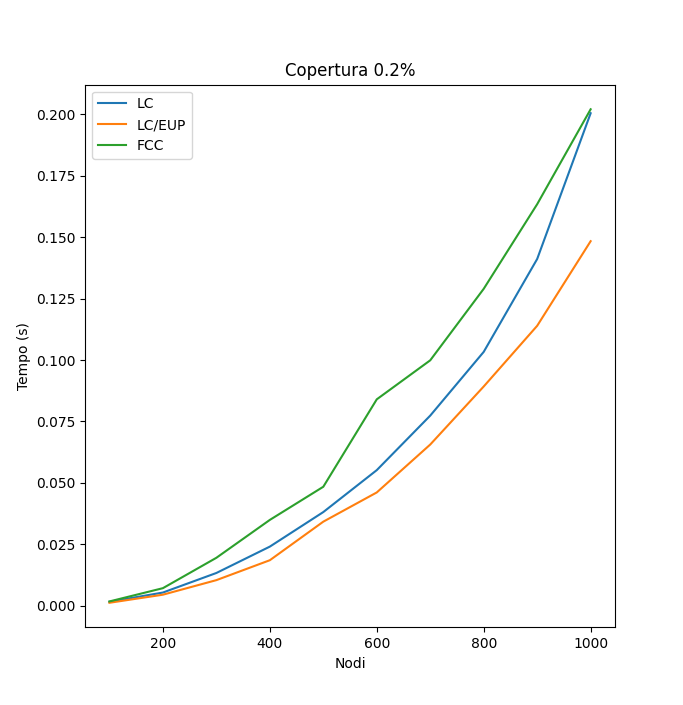
\includegraphics[width=\textwidth]{tests_results/cop0.2.png}
    \caption{Grafico dei tempi di esecuzione per la ricerca di componenti connesse in grafi non diretti con copertura 0.2\%}
\end{figure}


\begin{figure}
    \centering
    \captionsetup{justification=centering}
    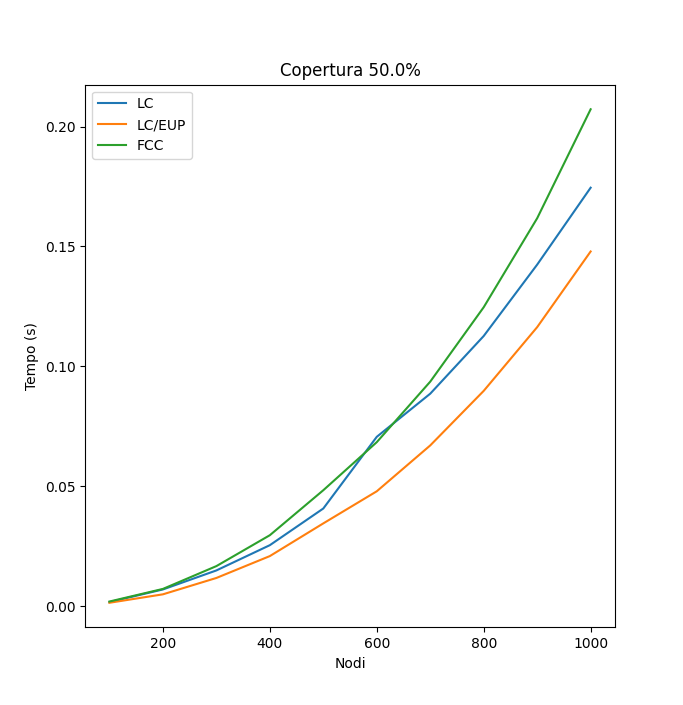
\includegraphics[width=\textwidth]{tests_results/cop50.png}
    \caption{Grafico dei tempi di esecuzione per la ricerca di componenti connesse in grafi non diretti con copertura 50\%}
\end{figure}


\begin{figure}
    \centering
    \captionsetup{justification=centering}
    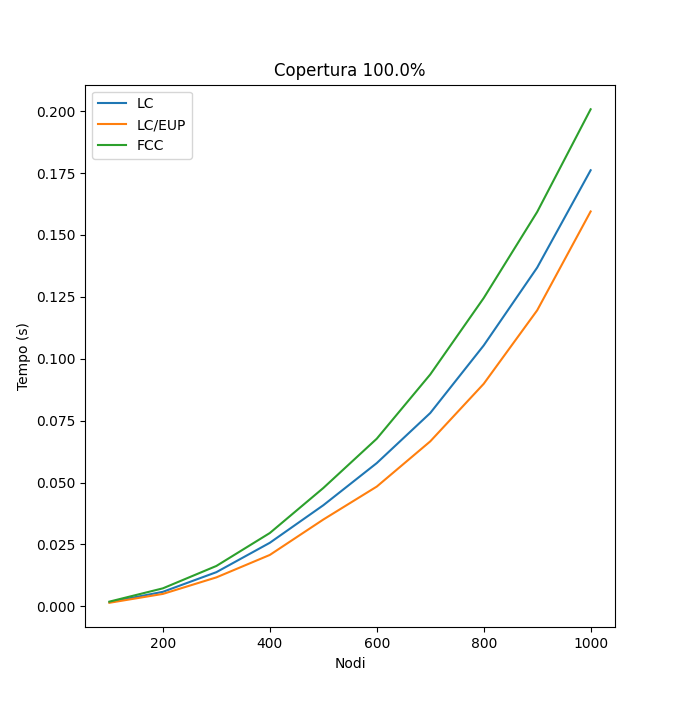
\includegraphics[width=\textwidth]{tests_results/cop100.png}
    \caption{Grafico dei tempi di esecuzione per la ricerca di componenti connesse in grafi non diretti con copertura 100\%}
\end{figure}
